\documentclass{zc-ust-hw}

\usepackage[]{lipsum} 

\name{SalahDin Ahmed Salh Rezk}
\id{202201079}
\course{Thermodynamics, Wave Motion and Optics}
\assignment{Assignment 3}

\usepackage{import}
\usepackage{xifthen}
\usepackage{pdfpages}

\newcommand{\incfig}[1]{%
    \def\svgwidth{\columnwidth}
    \import{./figures/}{#1.pdf_tex}
}

\begin{document}

\maketitle

\begin{enumerate}

  %%%%%%%%%%%%%
  \item Determine the minimum thickness of a quartz plate needed to convert a
    left-hand circularly polarized light source at a wavelength of $\lambda_0 = 656$ nm
    to right-hand circularly polarized light. The refractive indices for quartz
    are $n_s = 1.551$ and $n_f = 1.542$.
  %%%%%%%%%%%%%
    \begin{sol}
      Since the light is circularly polarized, the phase difference is $\pi$.
      \begin{align}
        \Delta\phi = \frac{2\pi}{\lambda_0} \Delta d \quad \Delta d = |n_s - n_f|d
      .\end{align}
      \begin{align}
        \pi &= \frac{2\pi}{\lambda_0} |n_s - n_f|d \\
        d &= \frac{\lambda_0}{2|n_s - n_f|} \\
          &= \frac{656 \times 10^{-9}}{2|1.551 - 1.542|} \\
          &= 3.6 \times 10^{-5} \text{ m}
      .\end{align}
    \end{sol}
  
  %%%%%%%%%%%%%
  \item For each of the provided electromagnetic waves, please characterize
    their polarization state and provide a rationale for your classification
  %%%%%%%%%%%%%
    \begin{enumerate}
      \item $E(z,t) = E_0\cos(k_0z-\omega_0t) \hat{x}-E_0\cos(k_0z-\omega_0t) \hat{y}$ 
        \begin{sol}
          Linearly polarized, because the electric field vector is constant in
          magnitude and direction.
        \end{sol}
      \item $E(z,t) = E_0\sin[2\pi(z\lambda^{-1}-v_0t)]\hat{x}-E_0\sin[2\pi(z\lambda^{-1}-v_0t)]\hat{y}$
        \begin{sol}
          Linearly polarized, because the electric field vector is constant in
          magnitude and direction.
        \end{sol}
      \item $E(z,t) = E_0\sin(\omega_0t-k_0z)\hat{x}+E_0\sin(\omega_0t-k_0z-\frac{\pi}{4})\hat{y}$
        \begin{sol}
          Elliptically polarized, because the electric field vector is constant
          in magnitude and varying in direction with phase difference of $\dfrac{\pi}{4}$.
        \end{sol}
      \item $E(z,t) = E_0\sin(\omega_0t-k_0z)\hat{x}+E_0\sin(\omega_0t-k_0z-\frac{\pi}{2})\hat{y}$
        \begin{sol}
          Circularly polarized, because the electric field vector is constant
          in magnitude and varying in direction with phase difference of $\dfrac{\pi}{2}$.
        \end{sol}
    \end{enumerate}

    \newpage

  %%%%%%%%%%%%%
  \item The index of refraction of air at 300 K and 1 atmosphere pressure is
    1.0003 in the middle of the visible spectrum. Assuming an isothermal
    atmosphere (of constant temperature) at 300 K, calculate by what factor the
    earth’s atmosphere would have to be denser to cause light to bend around
    the earth with the earth’s curvature at sea level. (In cloudless skies we
    could then watch sunset all night, in principle, but with an image of the
    sun drastically compressed vertically.) You may assume that the index of
    refraction $n$ has the property that $n - 1$ is proportional to the
    density. (Hint: Think of Fermat's Principle.) The $\frac{1}{e}$ height of
    this isothermal atmosphere is 8700 meters. (where $R = 6400 \times  10^3$ m
    is the earth's radius). i.e, $n(r)-1 = \rho e^{-\frac{r-R}{8700}}$.
  %%%%%%%%%%%%%

    \begin{figure}[ht]
      \centering
      \incfig{globe}
      \caption{}
      \label{fig:globe}
    \end{figure}

    \begin{sol}
      \begin{align}
        n(r) &= 1 + \rho e^{-\frac{r-R}{8700}} \\
        \frac{dn}{dr} &= -\frac{\rho}{8700} e^{-\frac{r-R}{8700}}
      .\end{align}
      \begin{align}
        l &= n(r)r\theta \\
        \frac{dl}{dr} &= \frac{dn}{dr}r\theta + n(r)\theta
      \end{align}
      \begin{equation}
        \implies \frac{dn}{dr}= -\frac{n(r)}{r}
      .\end{equation}
      \begin{equation}
        \frac{n(r)}{r} = \frac{\rho}{8700} e^{-\frac{r-R}{8700}}
      .\end{equation}
      \begin{equation}
        r=R=6.4\times 10^{6} \implies \frac{\rho \times 6.4\times 10^{6}}{8700} = 1 + \rho \implies \rho = 1.36 \times 10^{-3}
      \end{equation}
      \begin{equation}
        n_0 - 1 = \rho_0 \implies \rho_0 = 3 \times 10^{-4}
      .\end{equation}
      \begin{equation}
        \frac{\rho}{\rho_0} = \frac{1.36 \times 10^{-3}}{3 \times 10^{-4}} = 4.53
      \end{equation}
    \end{sol}

  %%%%%%%%%%%%%
  \item A rod of diameter d is bent to take the shape shown in the figure
    below. The inner radius of the curved part of the rod is denoted by $R$. Find
    the limiting value for $d/R$ for which all light rays entering normally at
    face $A$ of the rod will totally come out ONLY from face $B$. The refractive
    index of the material of the rod is 1.5.
  %%%%%%%%%%%%%

    \begin{figure}[ht]
      \centering
      \incfig{rod}
      \caption{}
      \label{fig:rod}
    \end{figure}

    \begin{figure}[htpb]
    \begin{center}
    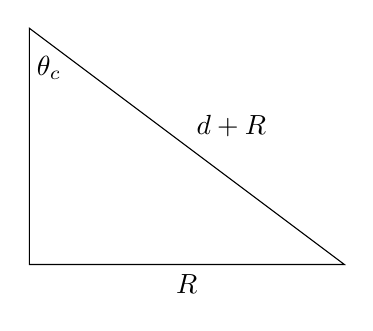
\begin{tikzpicture}[scale=1, transform shape]
      % Right angled triangle
      \draw (0,0) -- (0,3) -- node[above right]{$d+R$} (4,0) -- node[below]{$R$} cycle;
      % Angle at (0,3)
      \node at (0.25,2.5) {$\theta_c$};
    \end{tikzpicture}
    \end{center}
    \caption{}%
    \label{fig:triangle}
    \end{figure}

    \begin{sol}
      \begin{align}
        \sin\theta_c &= \frac{R}{d+R} \\
                     &= \frac{1}{n}
      .\end{align}
      \begin{align}
        \frac{d}{R} &= \frac{1}{\sin\theta_c} - 1 \\
                    &= \frac{1}{\frac{1}{n}} - 1 \\
                    &= n - 1
      .\end{align}
    \end{sol}

    \newpage

    %%%%%%%%%%%%%
  \item In the Figure~\ref{fig:a}, a light ray in an underlying material is
    incident at angle $\theta_1$ on a boundary with water, and some of the
    light refracts into the water. There are two choices of underlying
    material. For each, the angle of refraction $\theta_2$ versus the incident
    angle $\theta_1$ is given in the Figure~\ref{fig:b}. The horizontal axis
    scale is set by $\theta_{1s} = 90^{\circ}$. \\
    Without calculation, determine whether the index of refraction of (a)
    material 1 and (b) material 2 is greater or less than the index of water
    ($n = 1.33$). \\
    What is the index of refraction of (c) material 1 and (d) material 2?
    %%%%%%%%%%%%%

    \begin{figure}[H]
      \centering
      \begin{subfigure}[b]{.13333333333333333333\textwidth}
        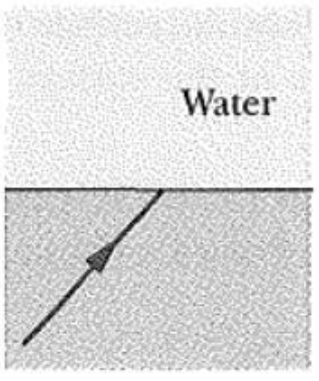
\includegraphics[width=\textwidth]{figures/a.png}
        \caption{}
        \label{fig:a}
      \end{subfigure}
      \begin{subfigure}[b]{0.2\textwidth}
        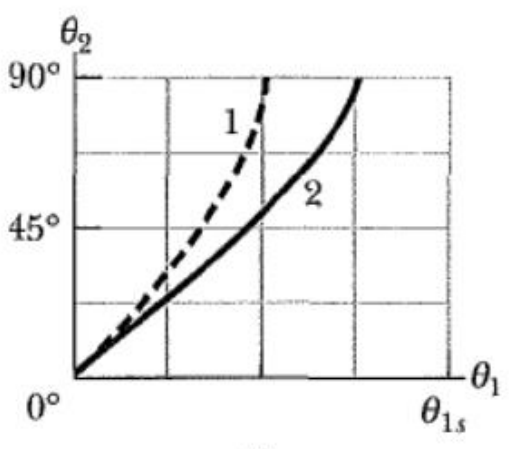
\includegraphics[width=\textwidth]{figures/b.png}
        \caption{}
        \label{fig:b}
      \end{subfigure}
      \caption{}
    \end{figure}

    \begin{sol}
      \begin{align}
        \theta_1 > \theta_2 \implies n_1 < n_2
      .\end{align}
      \begin{align}
        1.33\sin(45^{\circ}) &= n_1\sin(90^{\circ}) \\
        n_1 &= 1.33\sin(45^{\circ}) \\
            &= 1.33\frac{\sqrt{2}}{2} \\
        1.33\sin(67.5^{\circ}) &= n_2\sin(90^{\circ}) \\
        n_2 &= 1.33\sin(67.5^{\circ}) \\
            &= 1.33\frac{\sqrt{2+\sqrt{2}}}{2}
      .\end{align}
    \end{sol}

    \newpage

  \item A 4.00-m-long pole stands vertically in a lake having a depth of 2.00
    m. The Sun is 40.0$^{\circ}$ above the horizontal. Determine the length of the
    pole’s shadow on the bottom of the lake. Take the index of refraction for
    water to be 1.33. 

    \begin{figure}[ht]
      \centering
      \incfig{pole}
      \caption{}
      \label{fig:pole}
    \end{figure}

    \begin{sol}
      \begin{align}
        l_1 &= 2\cot\phi_1 \\
            &= 2\cot(40^{\circ}) \\
            &= 2.38\text{ m}
      .\end{align}
      \begin{align}
        1.33\sin\theta_2 &= \sin\theta_1 \\
        \theta_2 &= \sin^{-1}\left( \frac{\sin\theta_1}{1.33} \right) \\
                 &= \sin^{-1}\left( \frac{\sin(50^{\circ})}{1.33} \right) \\
                 &= 35.2^{\circ}
      .\end{align}
      \begin{align}
        l_2 - l_1 &= 2\cot(\theta_2) \\
                  &= 2\cot(35.2^{\circ}) \\
                  &= 2.84\text{ m}
      .\end{align}
      \begin{align}
        l_2 &= l_1 + 2.84 \\
            &= 5.22\text{ m}
      .\end{align}
    \end{sol}

\end{enumerate}

\end{document}
